\subsection{An application: There are graphs that are $(2, \infty)$-sided}

  We will show this by providing an example graph $G$ with a fixed corner assignment $\ext G$ we can do this due to Theorem \ref{th:fixCorner assignment}. Consider the graph in Figure \ref{fig:2manysidedLowerBound}. Note that most of the interior vertices are of degree $4$ and thus the largest part of any regular edge labeling is forced. Those edges that are forced to have a certain color are already colored in Figure \ref{fig:2manysidedLowerBound}.


  \begin{figure}[h!]
  \centering
  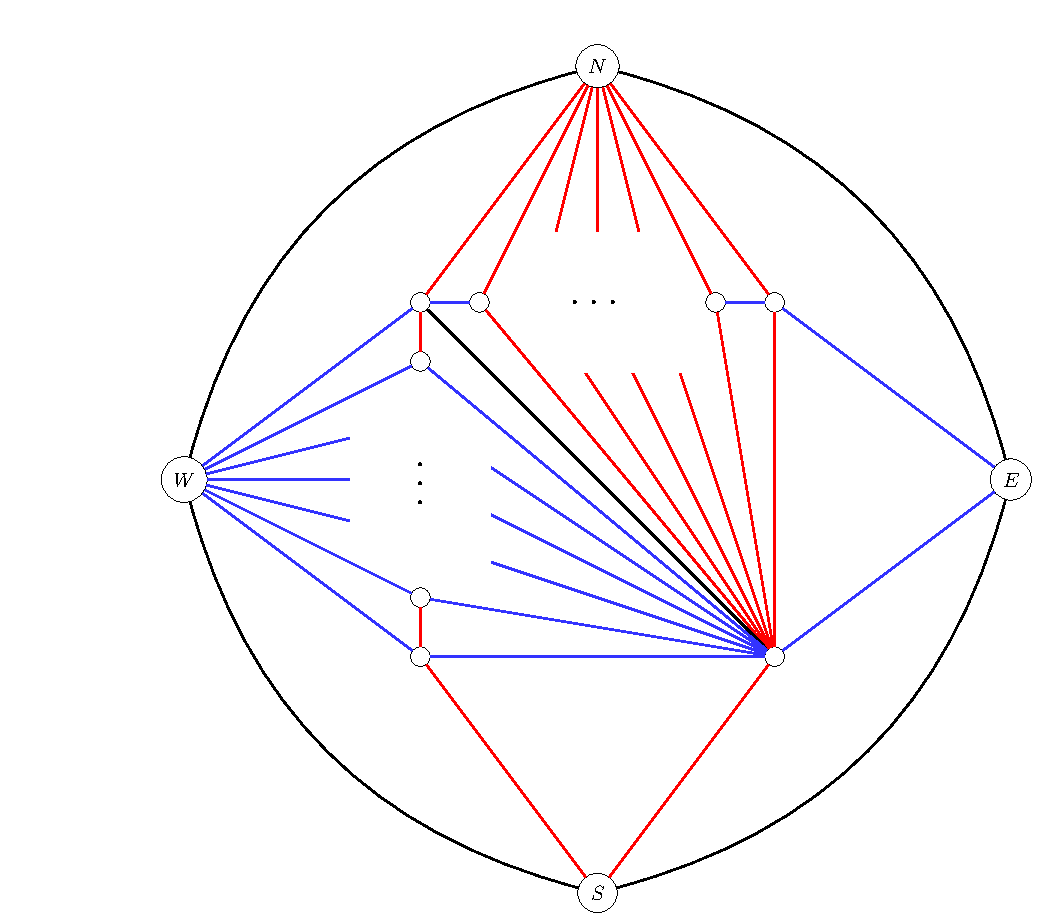
\includegraphics[scale=.5]{fixExtension/img/2manysidedLowerBound}

  \caption{The fixed corner assignment $\ext G$
      \label{fig:2manysidedLowerBound}}
  \end{figure}

  The only edge for which we have freedom to choose a color is the diagonal edge of $G$. However, if we color this edge blue we get a red $(2, \infty)$ cycle and if we color this edge red we get a blue $(2, \infty)$ cycle. In both cases we will thus obtain a maximal $(2,\infty)$-sided segment in our dual.
